\chapter{Voltage regulation}\label{ch:voltageRegulation}
%**********************************************

%**********************************************
\section{Introduction} \label{sec:voltIntro}
%**********************************************

The advantages and disadvantages of a linear regulator and a switchmode regulator will be explored in this chapter. While designing the regulator circuits, the specific datasheets for the LM7805 linear voltage regulator\cite{LM7805} and the LM2595 switchmode voltage regulator\cite{LM2595} was used to ensure the regulators are used with the correct capacitance, inductance, and resistance values. The variable voltage circuit required by the switchmode regulator\cite{LM2595} is a very incricate circuit, the calculations of which is described in the next section.

\begin{comment}Introduce the reader to what you want to present in this chapter. Include any references to literature you feel is needed. 
In this section, you put a very short summary of infrormation you gatherered from literature (papers, web sites, datasheets) that you used to do the design. Be sure to include the references, which you can add in the \texttt{References.bib} file. 

Some examples of how to cite (all in \texttt{References.bib}): 
It was stated by \cite{Booysen:2013} that ... . Subsequently, he changed his mind and said in  \cite{Gerber:2019} that ... .
While \cite{WebsiteOpAmp} claims it to be ... .
\end{comment}


%**********************************************
\section{Design} \label{sec:voltDesign}
%**********************************************

The voltage regulator must regulate a \SI{9}{VDC} supply to a stable \SI{5}{\volt} with little to no noise.\par
The LM7805 linear regulator circuit, as shown in Fig.\ref{subfig:linear_circuit_diagram}, is fairly simple. It is specified in \cite{LM7805} that the regulator requires an input capacitance of \SI{0.33}{\micro\F} and an output capacitance of \SI{0.1}{\micro\F} to improve the transient response. Bypass capacitors are recommended to improve stability, but as of writing the response of the regulator is favourable enough.\par
The LM2595 swicthmode regulator circuit, as shown in Fig.\ref{subfig:switchmode_circuit_diagram}, is more complex and requires more components. The chosen circuit as stated by \cite{LM2595} section 9.2.2 is a series buck regulator with adjustable output, of which the values of $C_{IN}$, $C_{OUT}$, $L_{1}$, and D1 are specified as \SI{120}{\micro\farad} 25-V electrolytic, \SI{120}{\micro\farad} 50-V electrolytic, \SI{100}{\micro\henry} and a 1N5822 3-A, 40-V Schottkey diode. The regulator is coupled with a Post Ripple filter, comprised of a series inductor of \SI{3}{\micro\henry} and a 15-V bypass capacitor of \SI{180}{\micro\farad}, to reduce ripple to half. This section includes the formulas needed to work out the values of the other components. $R_{1}$ is chosen as \SI{1}{\kilo\Omega} and $V_{REF}$ is specified as \SI{1.23}{\volt}.
\[
R_{2} = R_{1}(\frac{V_{OUT}}{V_{REF}}-1) =\SI{1}{\kilo\Omega}(\frac{\SI{5}{\volt}}{\SI{1.23}{\volt}}-1) = \SI{3.06}{\kilo\Omega} \approx  \SI{3}{\kilo\Omega}\]
\[C_{FF}=\frac{1}{31\times 10^3 \times R_2}= \frac{1}{31\times 10^3 \times \SI{3}{\kilo\Omega}}=\SI{10.75}{\nano\farad} \approx \SI{10}{\nano\farad}\]
\newline
To measure the voltage, current, power, and efficiency, the \texttt{LTSpice} function \texttt{.meas} is used (Fig.\ref{fig:measargs}).



\begin{comment}
In this section, you need to capture your design, which should include the following: 
\begin{itemize}
  \item Design rationale, i.e. what your thinking was behind the design.
  \item References to literature/sources as appropriate \cite{WebsiteOpAmp}.  
  \item You can assume the reader has an E\&E degree, and will not need detail explanations of trivial information (e.g. what a resistor is, or what Ohm's law is).  
  \item Design calculations, for example to determine resistor values and capacitor values, or to check for allowed voltage and current ranges and levels. These calculations should also give expected outputs, which hopefully matches the simulated values. 
  \item Analysis of given or expected input conditions. 
  \item Expected values and ranges based on your design. 
  \item Explain your choice of supply buy referring to the advantages and disadvantages of each. 
  \item Circuit diagram like the one in Figure \ref{fig:circuit_diagram}. I used ``print to PDF'' from LTSpice,  but feel free to use a cropped screengrab if you are PDF-challenged and do not have a PDF printer (there are some free PDF creators online). Also have a look at the demo video on SUNLearn. 
\end{itemize}

For your benefit, here is how to write values with units: \SI{150}{\milli\Omega} or \SI{199}{myUnits}, and this is how we write ranges: \numrange{2}{5} \si{\kilo\volt}.

Here is an inline equation $ \frac{55}{45+3}$. Here is a numbered equation in Eq. \ref{eq:myNumberedEquation}.
\begin{equation}
   a = \frac{55}{45+3}
   \label{eq:myNumberedEquation}. 
\end{equation}. 

\end{comment}


\begin{figure}
 \footnotesize
   \centering
   \begin{subfigure}[]{0.35\textwidth}
        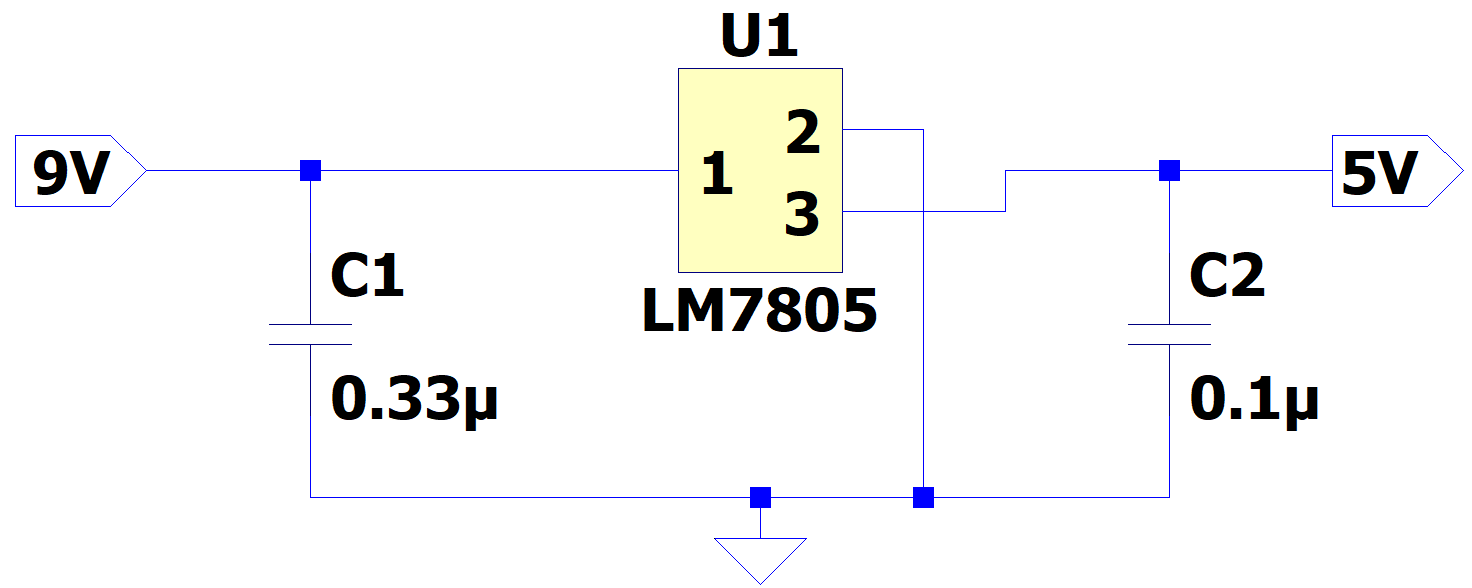
\includegraphics[width=\linewidth]{./Figures/Pictures/SpiceVoltRegLM7805.png}
	  \caption{Linear voltage regulator.} \label{subfig:linear_circuit_diagram}	
   \end{subfigure}
   \begin{subfigure}[]{0.55\textwidth}
  	 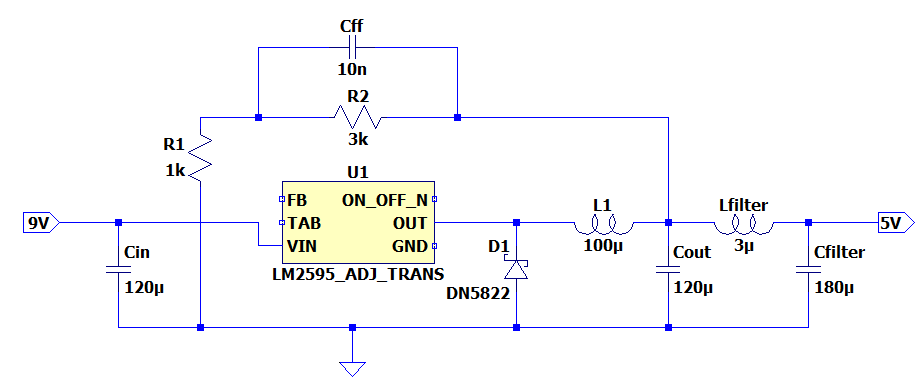
\includegraphics[width=\linewidth]{./Figures/Pictures/SpiceVoltRegLM2595.png}
	  \caption{Switchmode voltage regulator.} \label{subfig:switchmode_circuit_diagram}	
   \end{subfigure}
   
   \caption {Circuit diagrams of the two voltage regulators}.

      \label{fig:circuit_diagram}
 \end{figure}
%**********************************************
\section{Results} \label{sec:volt_results}
%**********************************************
\begin{comment}

In this section, you want to demonstrate, by means of referring to simulation results, using the designed circuit, how your circuit behaves as you designed it in Section \ref{sec:voltDesign}. Present and report on your simulated results in Figure \ref{fig:simulation_results_box} Be absolutely sure that the text and information in your report are readable. 

You can use screengrabs or photos of the oscilloscope, or download the CSVs and plot them as PDFs using Matlab, Excel or similar. 
You can also use tables, example of which are presented in Tables \ref{tab:table1} and \ref{tab:table2}.

\end{comment}

The voltage response for the two voltage regulators can be seen in Fig. \ref{fig:simulation_results_box}. The results are compared in Table \ref{tab:voltregresults}


\begin{figure}[H]
 \footnotesize
 \centering
    \begin{subfigure}[]{0.5\textwidth}
              \centering
  		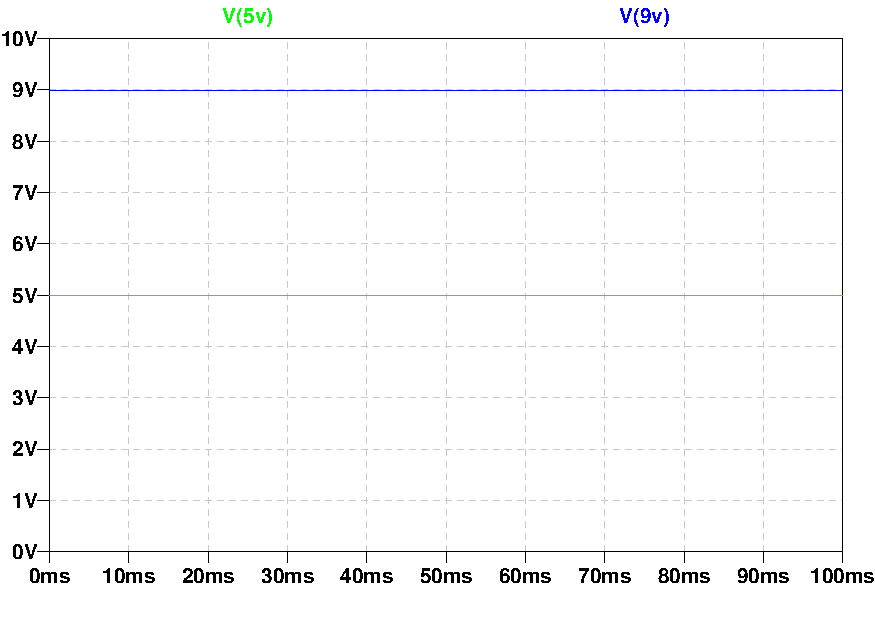
\includegraphics[width=1\linewidth]{./Figures/pdf/VoltRegLM7805Voltage.pdf}
		    \caption{} \label{subfig:linear_volt_response}
     \end{subfigure}
     \begin{subfigure}[]{0.4\textwidth}
             \centering
  		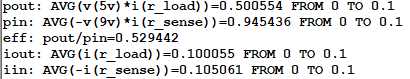
\includegraphics[width=1.0\linewidth]{./Figures/Pictures/VoltRegLM7805MeasResults}
		   \caption{ } \label{subfig:linear_meas_results}
     \end{subfigure}
    \begin{subfigure}[]{0.5\textwidth}
              \centering
  		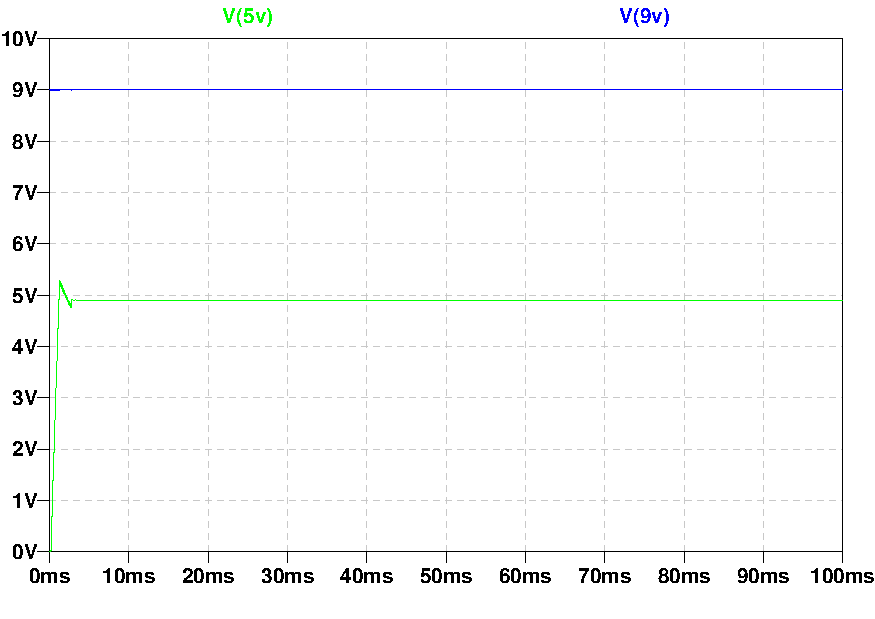
\includegraphics[width=1\linewidth]{./Figures/pdf/VoltRegLM2595Voltage.pdf}
		    \caption{} \label{subfig:swmd_volt_response}
     \end{subfigure}
    \begin{subfigure}[]{0.4\textwidth}
              \centering
  		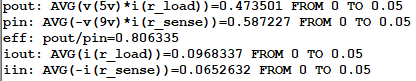
\includegraphics[width=1\linewidth]{./Figures/Pictures/VoltRegLM2595MeasResults}
		    \caption{} \label{subfig:swmd_meas_results}
     \end{subfigure}
   \caption[\textcolor{red}{I am the short caption that appears in the List of Figures list}]{Voltage regulation, comparing the linear and switchmode regulators... (a) Linear regulator voltage response (b) Linear Regulator \texttt{.meas} results.  (c)  Switchmode regulator voltage response (d) Switchmode regulator \texttt{.meas} results.}
    \label{fig:simulation_results_box}
 \end{figure}

\begin{figure}[H]
     \centering
     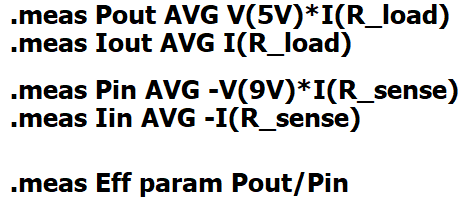
\includegraphics[width=0.35\linewidth]{./Figures/Pictures/VoltRegMeasureArguments.png}
     \caption{\texttt{.meas} arguments used in \texttt{LTSpice}}
     \label{fig:measargs}
 \end{figure}

\begin{table}[H]
        \centering
        \footnotesize
        \caption{Table of current, power and efficiency.}
         \begin{tabular}{c@{\qquad}rrrrrr}
          \toprule
             \multirow{2}{*}{} & \multicolumn{2}{c}{Current} & \multicolumn{2}{c}{Power}& Efficiency\\
          \cmidrule{2-5}
          & Supplied & Draw & Supplied & Draw &\\
          & [\SI{}{\milli\ampere}] & [\SI{}{\milli\ampere}]& [\SI{}{\milli\watt}]& [\SI{}{\milli\watt}]&[\%]\\
          \midrule
          LM7805 Linear & 105 & 100 & 945.44 & 500.55 & 52.94\\
          LM2595 Switchmode & 65.26 & 96.83 & 587.23 & 473.5 & 80.63 \\
          \bottomrule
        \end{tabular}
     \label{tab:voltregresults}
\end{table}

\begin{table}[H]
    \centering
    \footnotesize
    \captionsetup{justification=centering}
    \caption{Table of Absolute maximum ratings.\\ Based on the datasheet of LM7805 in \cite{LM7805} and LM2595 in\cite{LM2595} \\}
    \begin{tabular}{c@{\qquad}rrrr}
    \toprule
         & Maximum & Dropout Voltage  & Maximum \\
         & Allowed Input & at \SI{25}{\celsius} & Power Dissapation\\
         & [\SI{}{\volt}] & [\SI{}{\volt}]& [\SI{}{\watt}]\\
    \midrule
         LM7805 Linear & 30 & 1.7 & $\leq$ 0.75 \\
         LM2595 Switchmode & 45 & 0.88 & Limited Internally \\
    \bottomrule
    \end{tabular}
    \label{tab:max_ratings}
\end{table}

\begin{comment}
\begin{table}
         \centering
        \footnotesize
        \caption{Example of another table.}

         \begin{tabular}{c@{\qquad}rrrr}
          \toprule
          \multirow{2}{*}{\raisebox{-\heavyrulewidth}{Schools }} & \multicolumn{2}{c}{Total energy used}& \multicolumn{2}{c}{Change}\\
          \cmidrule{2-5}
            & 2017 & 2018 & $\Delta_{Abs}$ & $\Delta_{DiD}$\\
            & [kWh] & [kWh] & [\%] & [\%] \\
          \midrule
          A & 9,868      & 10,399 & +5 & -11\\
          B & 10,191     & 10,590 & +4 & -12\\
          \bottomrule
        \end{tabular}
     \label{tab:table2}
\end{table}
\end{comment}

\par
From the figures and tables it is seen that both regulators have advantages and disadvantages. \newline
The LM7805 regulator has a more favourable response, a higher dropout voltage, and less expensive components, but is not very efficient in terms of power.\newline
The LM2595 regulator is much more efficient and higher maximum allowed input, but is much more expensive in terms of components and circuit real estate, and only alows us to reach the desired output after a certain time.
As for maximum ratings, the LM7805 linear regulator has a high enough power ceiling that it won't cause any problems for our circuit.

%**********************************************
\section{Summary}\label{sec:temp_summary_ch2}
%**********************************************
From the results, the chosen design is the LM7805 linear regulator. Although not as efficient, it is less expensive, has a higher dropout voltage and better voltage response, which is important for it's use with a temperature sensor, where noise is already a big problem.


